\section{Experiment 1: Analyzing Performance of TCP Variants}
This experiment analyzed the performance of different TCP variants over a setup consisting of a single TCP stream and a single CBR flow. The performance of the TCP variants were analyzed over a range of different packet sizes and transmission rates assigned to the CBR. We analyze the results of this experiment in two parts. First, by looking at the performance of the variants over an increasing range of CBR packet sizes, while the rate of the link is constant at 2Mbps. Second, we look at the performance of the variants over an increasing range of tranmission rates - from 1Mbps to 10Mbps, while the size of the packet is held constant at 3,000 bytes.

When holding the transmission rate steady, at 2Mbps, none of the variants experienced any packet loss over the range of increasing packet sizes, from 500 bytes to 8,000 bytes. The average and end-to-end latency as well as the throughput for TCPs Vegas, Reno, NewReno and Tahoe were all the same. This is consistent with the fact that these variants differ only in the ways they retransmit lost packets. 

Vegas keeps the link as fully saturated as possible, to achieve higher bandwidth utilization. Given no congestion TCP Vegas maintains a higher throughput than TCPs Reno, NewReno and Tahoe. 

\begin{figure}[!htbp]
	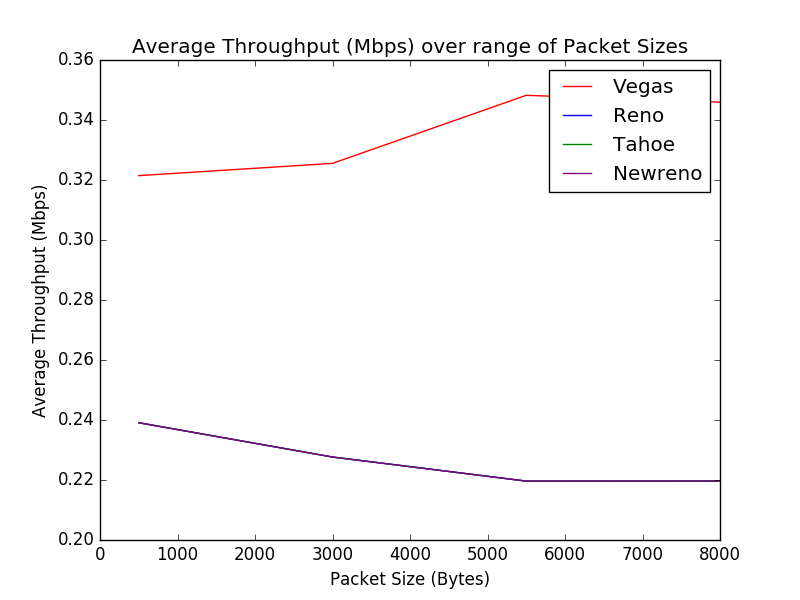
\includegraphics[scale=0.4]{P1.png}
	\caption{TCP Vegas (red) maintains a higher throughput than TCPs Reno, NewReno, and Tahoe (all purple) in a network with no congestion.}
	\label{a:label}
\end{figure}

In a network with congestion, TCP Vegas takes preventative measures in avoiding it. The other variants make changes only in the aftermath of packet loss. To prevent congestion, Vegas records the round trip time (RTT) of packets and adjusts its congestion window according to any delay. As shown in Figure 2, TCPs Reno, NewReno and Tahoe experience their first packet loss when the CBR rate is set to 6Mbps. Vegas does not experience packet loss until the CBR rate is 9Mbps.

\begin{figure}[!htbp]
	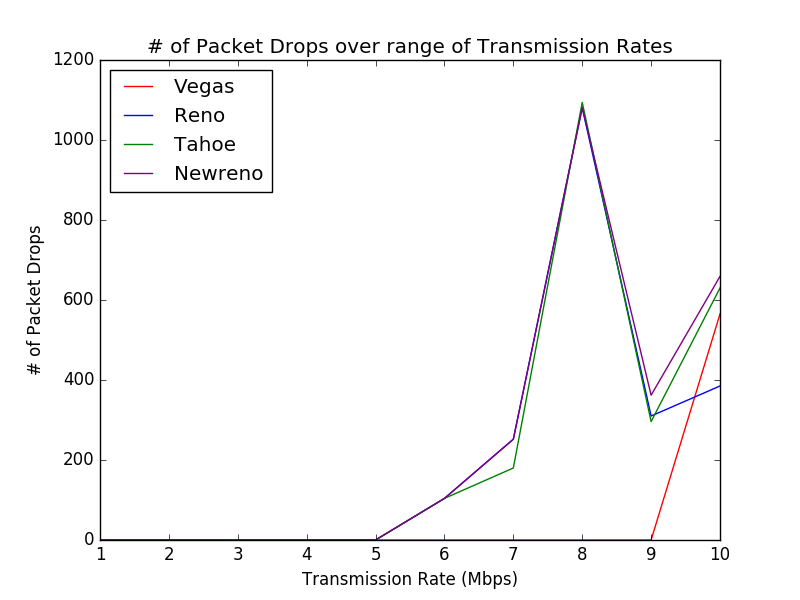
\includegraphics[scale=0.4]{PDrops.png}
	\caption{This figure shows the number of packet drops when the CBR flow has a rate of 10Mbps and the packet size is increasing.}
	\label{a:label}
\end{figure}

Despite packet loss occuring at a rate of 9Mbps in TCP Vegas, Figure 3 shows the throughput decreasing, before experiencing packet loss. This is because Vegas is sensing the increased congestion on the network as a result of increasing RTTs and decreasing its congestion window accordingly as a preventative measure, before experiencing packet loss. As a result, the latency also increased.

\begin{figure}[!htbp]

	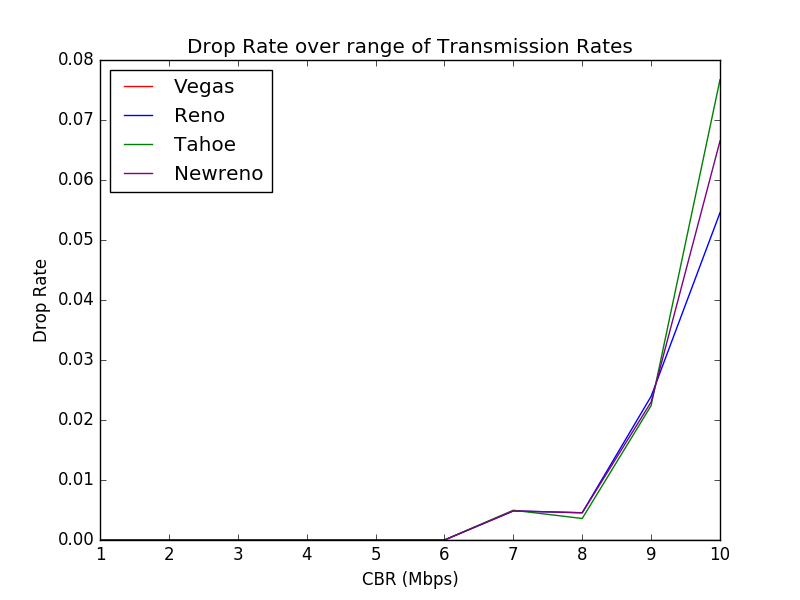
\includegraphics[scale=0.4]{P2.png}
	\caption{Throughputs of each of the TCP Variants as the CBR flow rate increases, causing contention.}
	\label{a:label}
\end{figure}

Each variant is consistent, only in that they wait until receiving 3 duplicate-acknowledgements or retransmit timeouts before retransmitting the first lost packet. Given a network with a single TCP variant, which experiences little congestion, TCP Vegas experiences higher throughput and lower latency. 

Given low-to-moderate levels of congestion, TCP Vegas is able to efficiently decrease its congestion window size, before experiencing packet loss, and thus is able to maintain 0 packet loss while its counterparts are unable to. However, once some threshhold is reached, for example a CBR flow rate of 10Mbps in our experiments, Vegas inevitabley suffers packet loss, and at this point it is no longer the most efficient variant in terms of dealing with loss. NewReno, handles multiple packet losses better than its counterparts. After the first packet loss is identified by a triple duplicate acknowledgement, or by a retransmission timeout, NewReno assumes that any packet following a partial acknowledgment is lost. This makes the retransmission of packets much faster and accounts for the increase in throughput experienced by NewReno in Figure 3. Given moderate to high amounts of congestion, NewReno has higher throughputs and lower latency than the other variants.


